\documentclass[10pt]{article}
\usepackage[a4paper,landscape,margin=12mm]{geometry}
\usepackage{tikz}
\usetikzlibrary{arrows.meta}
\pagestyle{empty}

\definecolor{ink}{HTML}{203449}
\definecolor{edge}{HTML}{53687E}
\definecolor{blue}{HTML}{245B8D}
\definecolor{green}{HTML}{22634A}
\definecolor{amber}{HTML}{80520E}
\tikzset{
    box/.style={draw=edge, fill=white, rounded corners=3pt, align=center,
        text=ink, minimum height=11mm, minimum width=37mm, font=\small},
    payment/.style={box, draw=blue, fill=blue!8},
    role/.style={box, draw=green, fill=green!8},
    tool/.style={box, draw=amber, fill=amber!8},
    frame/.style={rounded corners=5pt, draw=edge!55, fill=edge!4},
    wire/.style={draw=edge, line width=.7pt, rounded corners=2pt},
    flow/.style={wire, -{Stealth[length=2mm]}},
    label text/.style={font=\scriptsize, text=ink, fill=white, inner sep=2pt},
    title/.style={font=\large\bfseries, text=ink, anchor=west, inner sep=0pt}
}

\begin{document}
\sffamily
\noindent\makebox[\textwidth][c]{%
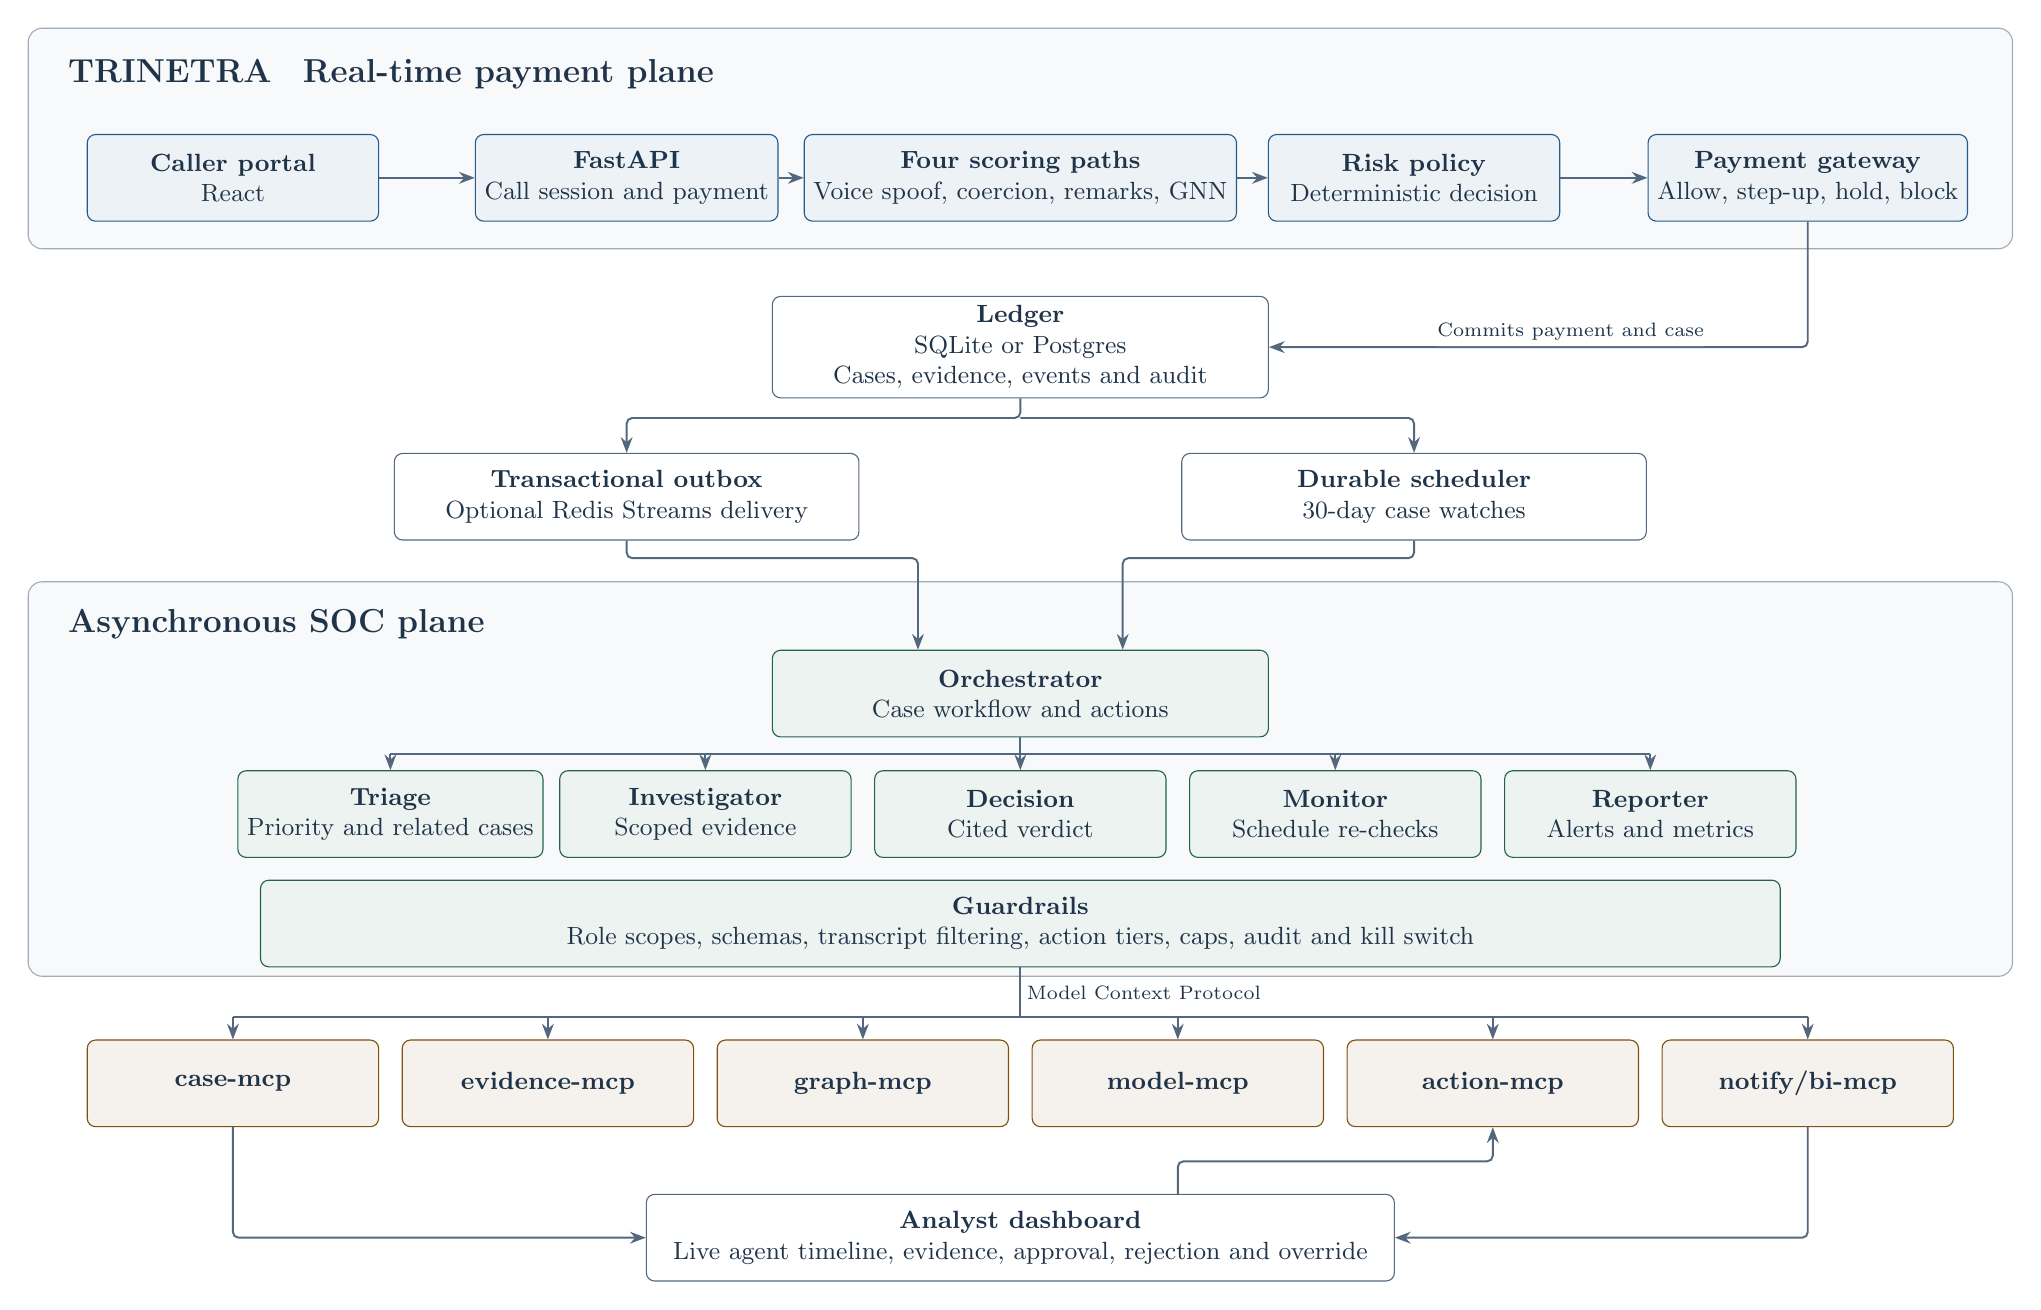
\begin{tikzpicture}
    \draw[frame] (-12.6,-.9) rectangle (12.6,1.9);
    \node[title] at (-12.1,1.32) {TRINETRA \enspace Real-time payment plane};
    \node[payment] (portal) at (-10,0) {\textbf{Caller portal}\\React};
    \node[payment] (api) at (-5,0) {\textbf{FastAPI}\\Call session and payment};
    \node[payment] (scores) at (0,0) {\textbf{Four scoring paths}\\Voice spoof, coercion, remarks, GNN};
    \node[payment] (policy) at (5,0) {\textbf{Risk policy}\\Deterministic decision};
    \node[payment] (gateway) at (10,0) {\textbf{Payment gateway}\\Allow, step-up, hold, block};
    \draw[flow] (portal) -- (api);
    \draw[flow] (api) -- (scores);
    \draw[flow] (scores) -- (policy);
    \draw[flow] (policy) -- (gateway);

    \node[box, minimum width=63mm] (ledger) at (0,-2.15)
        {\textbf{Ledger}\\SQLite or Postgres\\Cases, evidence, events and audit};
    \node[box, minimum width=59mm] (outbox) at (-5,-4.05)
        {\textbf{Transactional outbox}\\Optional Redis Streams delivery};
    \node[box, minimum width=59mm] (scheduler) at (5,-4.05)
        {\textbf{Durable scheduler}\\30-day case watches};
    \draw[flow] (gateway.south) |- node[pos=.72,label text,above] {Commits payment and case} (ledger.east);
    \draw[flow] (ledger.south) -- (0,-3.05) -| (outbox.north);
    \draw[flow] (0,-3.05) -| (scheduler.north);

    \draw[frame] (-12.6,-10.14) rectangle (12.6,-5.13);
    \node[title] at (-12.1,-5.67) {Asynchronous SOC plane};
    \node[role, minimum width=63mm] (orchestrator) at (0,-6.55)
        {\textbf{Orchestrator}\\Case workflow and actions};
    \node[role] (triage) at (-8,-8.08) {\textbf{Triage}\\Priority and related cases};
    \node[role] (investigate) at (-4,-8.08) {\textbf{Investigator}\\Scoped evidence};
    \node[role] (decide) at (0,-8.08) {\textbf{Decision}\\Cited verdict};
    \node[role] (monitor) at (4,-8.08) {\textbf{Monitor}\\Schedule re-checks};
    \node[role] (report) at (8,-8.08) {\textbf{Reporter}\\Alerts and metrics};
    \node[role, minimum width=193mm] (guards) at (0,-9.47)
        {\textbf{Guardrails}\\Role scopes, schemas, transcript filtering, action tiers, caps, audit and kill switch};
    \draw[flow] (outbox.south) -- (-5,-4.83) -| ([xshift=-13mm]orchestrator.north);
    \draw[flow] (scheduler.south) -- (5,-4.83) -| ([xshift=13mm]orchestrator.north);
    \draw[wire] (orchestrator.south) -- (0,-7.32);
    \draw[wire] (-8,-7.32) -- (8,-7.32);
    \foreach \agent/\pos in {triage/-8,investigate/-4,decide/0,monitor/4,report/8} {
        \draw[flow] (\pos,-7.32) -- (\agent.north);
    }

    \node[tool] (caseMcp) at (-10,-11.5) {\textbf{case-mcp}};
    \node[tool] (evidenceMcp) at (-6,-11.5) {\textbf{evidence-mcp}};
    \node[tool] (graphMcp) at (-2,-11.5) {\textbf{graph-mcp}};
    \node[tool] (modelMcp) at (2,-11.5) {\textbf{model-mcp}};
    \node[tool] (actionMcp) at (6,-11.5) {\textbf{action-mcp}};
    \node[tool] (notifyMcp) at (10,-11.5) {\textbf{notify/bi-mcp}};
    \draw[wire] (guards.south) -- node[label text, right] {Model Context Protocol} (0,-10.66);
    \draw[wire] (-10,-10.66) -- (10,-10.66);
    \foreach \toolname/\pos in {caseMcp/-10,evidenceMcp/-6,graphMcp/-2,modelMcp/2,actionMcp/6,notifyMcp/10} {
        \draw[flow] (\pos,-10.66) -- (\toolname.north);
    }

    \node[box, minimum width=95mm] (console) at (0,-13.46)
        {\textbf{Analyst dashboard}\\Live agent timeline, evidence, approval, rejection and override};
    \draw[flow] (caseMcp.south) |- (console.west);
    \draw[flow] (notifyMcp.south) |- (console.east);
    \draw[flow] ([xshift=20mm]console.north) |- (6,-12.49) -- (actionMcp.south);
\end{tikzpicture}%
}
\end{document}
